\chapter{\ifenglish Background Knowledge and Theory\else ทฤษฎีที่เกี่ยวข้อง\fi}

% การทำโครงงาน เริ่มต้นด้วยการศึกษาค้นคว้า ทฤษฎีที่เกี่ยวข้อง หรือ งานวิจัย/โครงงาน ที่เคยมีผู้นำเสนอไว้แล้ว ซึ่งเนื้อหาในบทนี้ก็จะเกี่ยวกับการอธิบายถึงสิ่งที่เกี่ยวข้องกับโครงงาน เพื่อให้ผู้อ่านเข้าใจเนื้อหาในบทถัดๆ ไปได้ง่ายขึ้น

\section{ทฤษฎีที่เกี่ยวข้อง}
\subsection{องค์ประกอบเกมสยองขวัญ} \cite{component-horror:theory} องค์ประกอบที่สำคัญมี ดังนี้
\begin{enumerate}
  \item เสียงและเพลงประกอบ เป็นส่วนประกอบหลักๆ ของการสร้างความสยองขวัญให้กับผู้เล่น ยกตัวอย่างเช่น เสียงพระสวดหรือดนตรีไทย ในเกม Home Sweet Home เป็นต้น
  \item ตัวละครที่ไร้ทางสู้ เป็นการเพิ่มความกดดันให้กับผู้เล่น เช่น สาวตาบอดหนีฆาตกรโรคจิตในเกม perception
  \item สถานที่ปิดตาย อาทิ ยานอาวกาศหรือจะเป็นโลกที่ถูกสร้างขึ้นมาอย่างบิดเบี้ยว สร้างความอึดอัด ไร้ทางหนี
  \item เรื่องราวที่มาที่ไปของความหายนะ ทุกๆเรื่องของความสยองขวัญ ต้องมีที่มาที่ไป เพื่อช่วยให้ผู้เล่นรู้สึกสยองขวัญ
  \item การแก้ไขปริศนา เกมแนวสยองขวัญเกือบจะทุกเกมนั้นต้องมีการแก้ไขปริศนาเพื่อหากุญแจที่จะนำมาเปิดประตู หรือหาสิ่งของมาเพื่อนำไปกระทำอะไรบางอย่าง เพื่อที่จะทำให้เราสามารถไปต่อได้
  \item เหยื่อผู้ร่วมชะตากรรม การเพิ่มตัวละครผู้เคราะห์ร้าย ที่อาจจะรอดหรือไม่รอดทำใ้หเราลุ้นจนจบ
  \item สิ่งของ อุปกรณ์ในการเอาตัวรอด ช่วยให้เราเอาตัวรอด บางอย่างก็เป็นอุปกรณ์ที่ใช้เเจ้งเตือนถึงบางสิ่งที่ไม่ประสงค์ดี
  \item เป้าหมาย เงื่อนไขที่เราต้องอยู่ที่แห่งนั้น เกมจำเป็นต้องมีเป้าหมาย เพื่อเป็นตัวกำหนดของการกระทำต่อๆไปของผู้เล่น
  \item อยู่ถูกที่ถูกเวลาหรือตรงตามเงื่อนไขที่ตัวร้ายกำหนด ตัวละครที่เราเป็นผู้เล่น เข้าไปติดกับดัก แล้วพบกับฆาตกรแบบพอดิบพอดี
\end{enumerate}

\section{เกมที่เกี่ยวข้อง}
\subsection{The Coma 2: Vicious sisters}
\subsubitem \textbf{The Coma 2:Vicious sisters} \cite{the-coma-2:theory} เป็นเกมแนว Survival Horror โดยผู้เล่นจะรับบทเป็นนักเรียนสาว พักมินอา ที่ตื่นขึ้นมาในโรงเรียนตอนดึก เธอได้รับรู้ถถึงสิ่งที่ผิดปกติ เธอพบว่ามีใครบางคนกำลังทำบางอย่าง ที่หน้าตาเหมือนอาจารย์ของเธอ พุ่งเข้ามาทำร้าย เธอจึงต้องหลบหนีเพื่อไม่ให้ถูกจับตัว โดยหนีไปในที่ที่ห่างออกไป แล้วพบกับสิ่งที่ทำให้ประหลาดใจมากมาย รวมไปถึงผู้ร่วมทางที่ดูไม่ค่อยเป็นมิตร จุดดเด่นของเกมนี้คือจะให้ผู้เล่นคอยหลบหนี จากการถูกจับตัว และจะมีสิ่งของให้ใช้เพื่อการอยู่รอด
\begin{figure}[h]
  \centering
  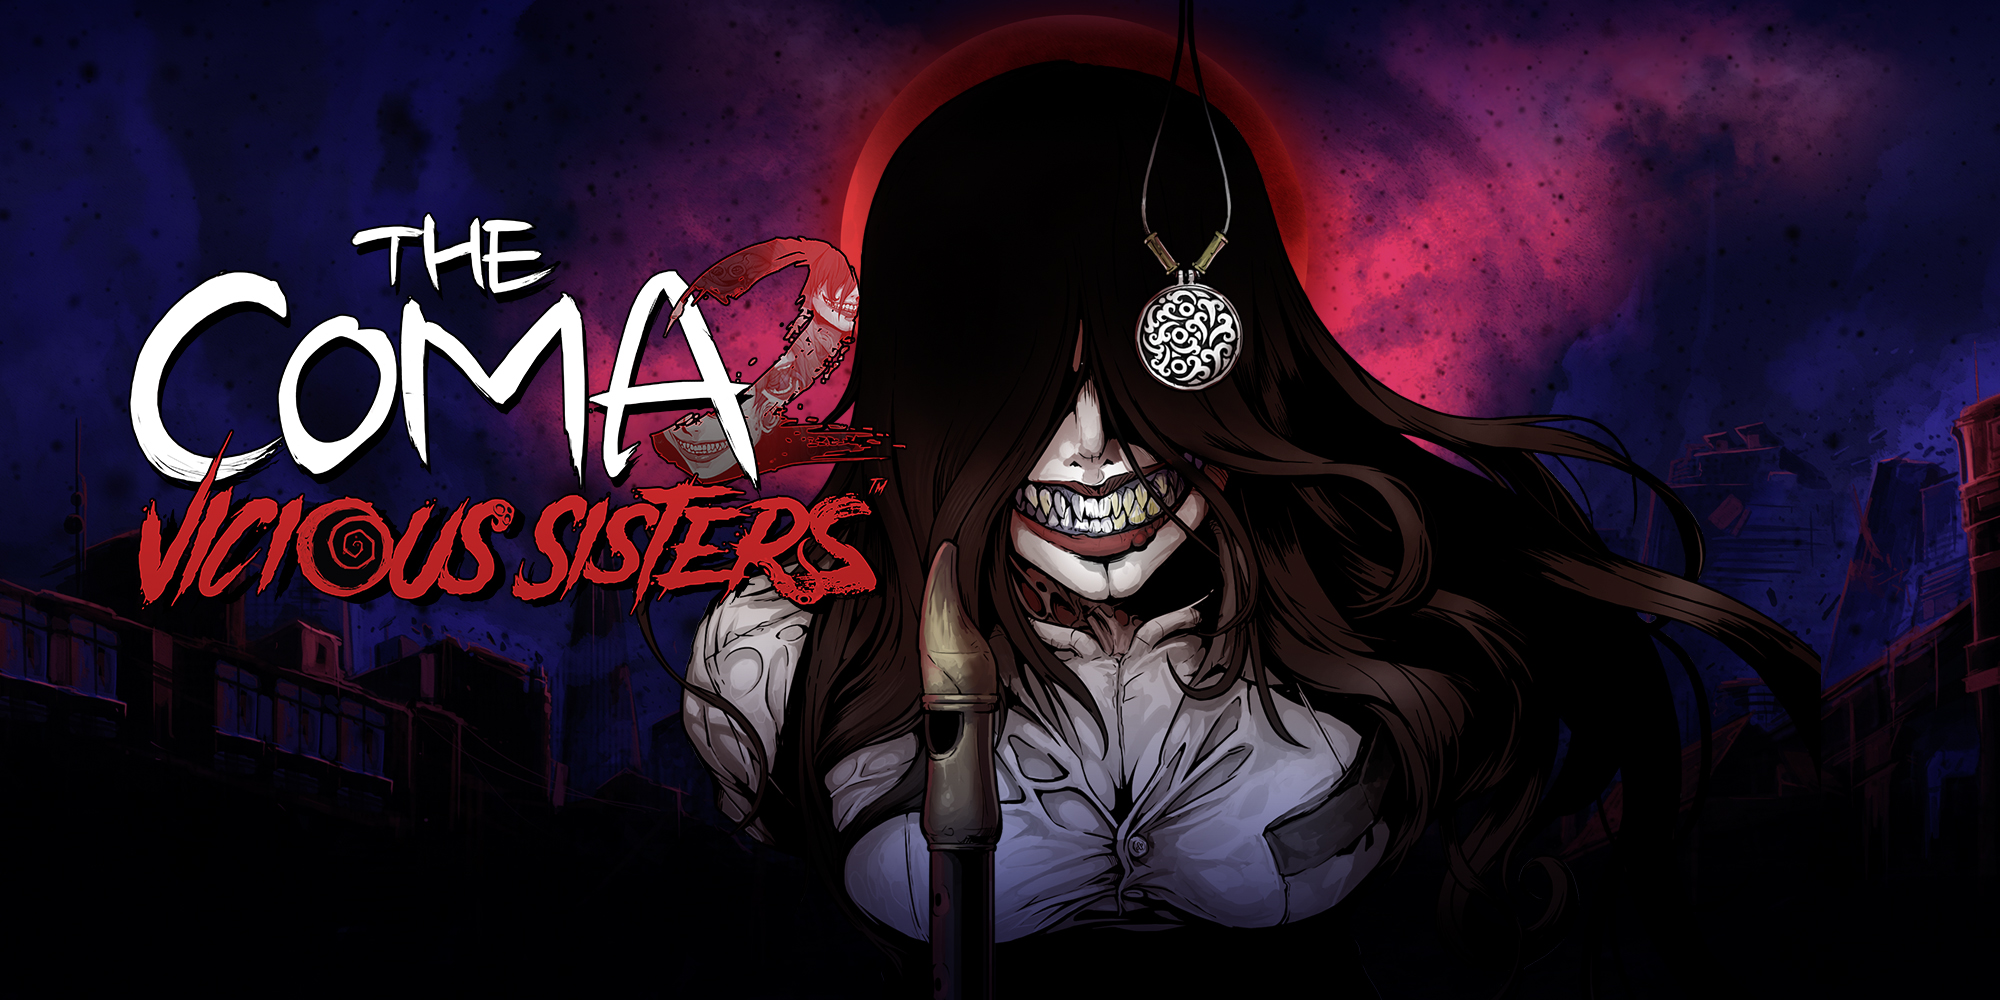
\includegraphics[width=0.6\textwidth, height=0.2\textheight]{Images/H2x1_NSwitchDS_TheComa2ViciousSisters.jpg}
  \caption{The Coma 2: Vicious sister จากเว็บไซต์}\label{TheComa2ViciousSisters}
\end{figure}

\subsection{Home Sweet Home}
\subsubitem \textbf{Home Sweet Home} \cite{home-sweet-home:theory} เป็นเกมแนว First Person, Adventure-Puzzle Horror โดยผู้เล่นจะรับบทเป็น ติม ที่ตื่นขึ้นมาในหอพักที่ไม่รู้จักมาก่อน เขาจึงออกสำรวจ แล้วได้เจอกับนักศึกษาสาว ที่อยู่ดีๆก็เข้ามาทำร้าย ทำให้ติมต้องหลบหนีออกจากหอพักแห่งนี้ ในระหว่างทางเขาได้พบกับเบาะแสบางอย่างที่ยังเป็นปริศณา หลังจากที่เขาได้หลบหนีออกมาได้ ติมก็ได้รู้สึกตัวอยู่ที่บ้านของเขา และได้รับสายฝากข้อความจากภรรยาของเขา เจน เจนได้หายตัวไป และได้ฝากไดอารี่ทิ้งไว้ ทำให้ติมต้องออกไปตามหาเจน ที่ระหว่างทางก็ได้พบกับเรื่องราวแปลกๆมากมาย ปริศณาว่าเจนอยู่ที่ไหน จุดเด่นของเกมจะเน้นไปที่การเล่าเรื่องราว และการหลบหนี/ซ่อนตัว จากภูติผีต่างๆที่จะมาออกล่า
\begin{figure}[h]
  \centering
  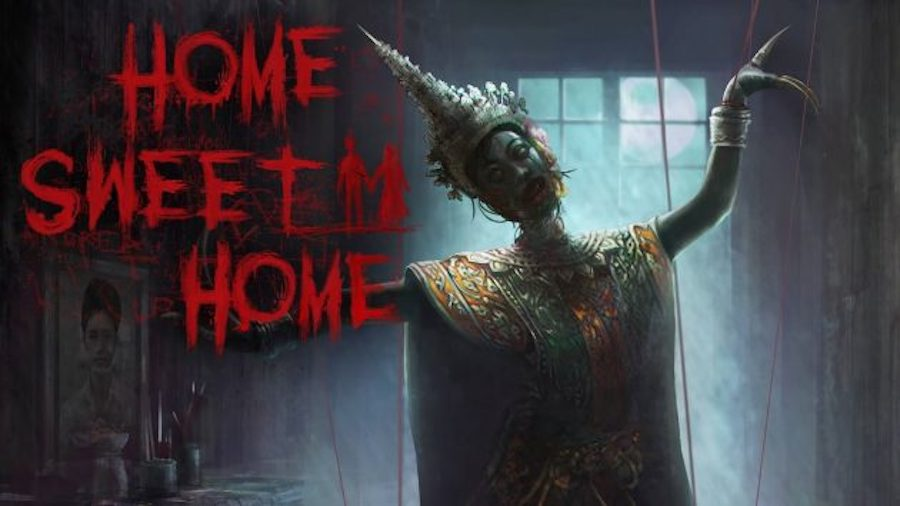
\includegraphics[width=0.6\textwidth, height=0.2\textheight]{Images/800px-HomeSweetHomePoster1.jpg}
  \caption{Home Sweet Home จากเว็บไซต์}\label{HomeSweetHomePoster1}
\end{figure}

\subsection{Outlast}
\subsubitem \textbf{Outlast} \cite{outlast:theory} เป็นเกมแนว First Person, Survival Horror โดยผู้เล่นจะรับบทเป็น Miles Upshur นักข่าวอิสระที่ได้รับข้อมูลจากแหล่งที่ไม่เปิดเผยตัวตน เขาจึงได้ลักลอบเข้าไปยัง Mount Massive Asylum บ้านร้างสำหรับคนป่าวโรคจิต และเขาก็ได้พบกับสิ่งที่น่าสะพรึงกลัวทั้งการทดลองที่ผิดจริยธรรมกับมนุษย์ ศาสนาที่บิดเบี่ยว วิญญาณผู้ป่วยทางจิต เขาจึงต้องหาทางออกไปจากสถานที่แห่งนี้ และนำเรื่องราวออกสู่โลกภายนอก จุดเเด่นของเกมนี้ ผู้เล่นจะต้องหาสิ่งของต่างๆ เพื่อนำมาปลดล็อคเส้นทางที่จะนำไปสู่การหลุดพ้น ผู้เล่นจะได้ใช้กล้องเพื่อบันทึกสิ่งต่างๆเพื่อเก็บข้อมูลที่จะคอยเฉลยเรื่องราวไปทีละส่วนๆ ผู้เล่นจะต้องคอยหลบซ่อนจากผู้ป่วยทางจิตและวิญญาณ
\begin{figure}[h]
  \centering
  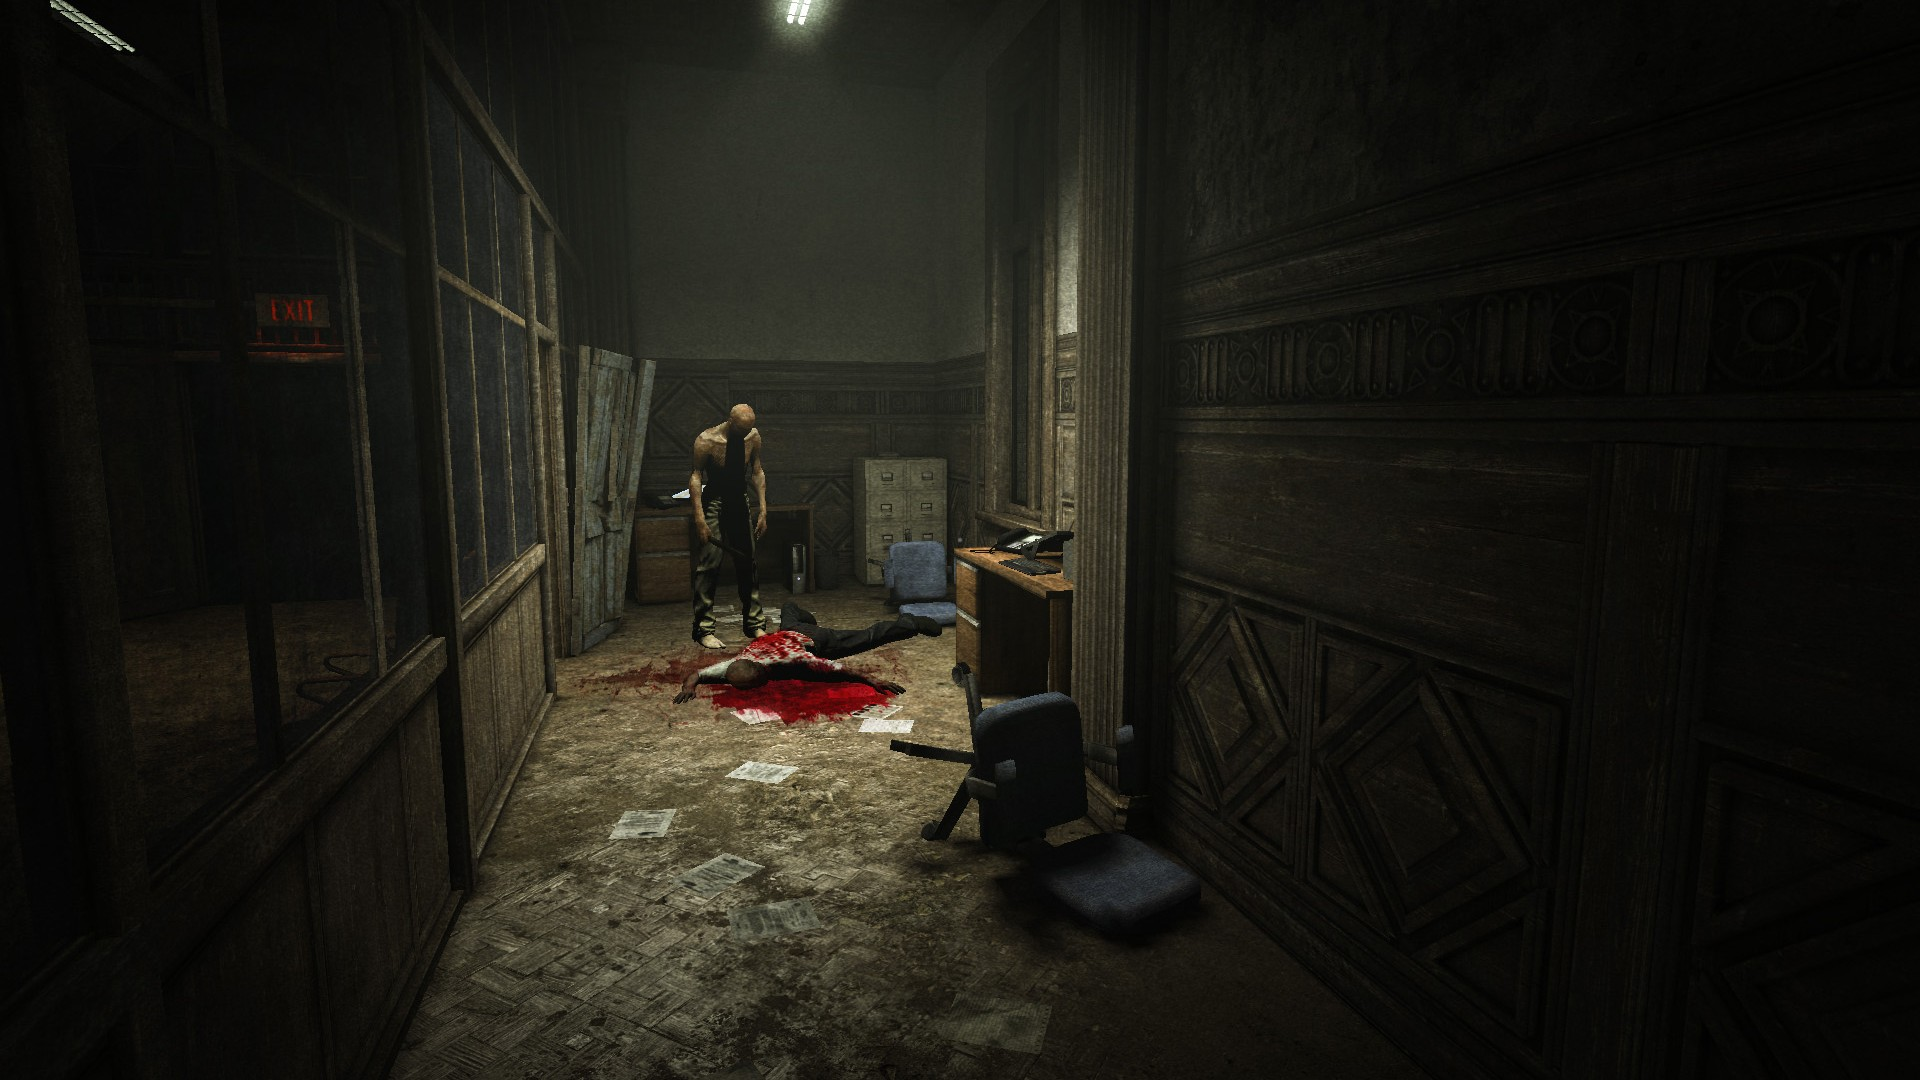
\includegraphics[width=0.6\textwidth, height=0.2\textheight]{Images/OutlastScreenShot-04-1920x1080.jpg}
  \caption{Outlast จากเว็บไซต์}\label{OutlastScreenShot}
\end{figure}

\subsection{Little Misfortune}
\subsubitem \textbf{Little Misfortune} \cite{outlast:theory} เป็นเกมประเภท side scrolling ซึ่งผู้เล่นจะได้รับบทเป็นหนูน้อย Little Misfortune ที่เป็นเด็กหญิงที่มีความมองโลกในแง่ดี เป็นคนสดใสร่าเริง ชอบแจกความสดใสโดยการโปรยกากเพชรใส่สิ่งของต่าง ๆ หนูน้อยจะออกเดินทางไปในเมืองซึ่งจะมีผู้ที่พูดคุยด้วย นั่นก็คือ Mr.Voice เขาจะนำทางหนูน้อยไปในที่ต่าง ๆ ซึ่งแรกๆก็ดูเหมือนจะเป็นเกมผจญภัยที่มีภาพน่ารักเหมือนการ์ตูนสำหรับเด็ก แต่เนื้อเรื่องกลับแฝงไปด้วยเนื้อหาของความบิดเบี้ยวของมนุษย์ ซึ่งประวัติของหนูน้อย Little Misfortune ก็คือเป็นเด็กที่เกิดมาโดยการท้องไม่พร้อม อีกทั้งยังมีความรุนแรงทางเพศและการใช้ภาษา การใช้ยาเสพติด เช่น บุหรี่ ซึ่งเป็นภาพที่หนูน้อยเห็นทุกวันจากแม่ที่ติดบุหรี่ และ Mr.Voice ที่หวังจะกลืนกินวิญญาณของหนูน้อยคนนี้ จึงหลอกเธอว่าเป็นเพื่อนที่ดี แต่ในโชคร้ายก็ยังมีโชคดีก็คือมีหมาจิ้งจอกตัวหนึ่งที่คอยช่วยเหลือหนูน้อยจาก Mr.Voice และในตอนจบของเรื่องก็ได้มีการเฉลยว่า อันที่จริงแล้ว หนูน้อย Little Misfortune ได้เสียชีวิตตั้งแต่เดินออกจากประตูบ้านไปแล้ว และคำว่า Little Misfortune ที่เธอใช้เรียกแทนตัวเอง ก็เป็นเพราะว่าตั้งแต่เธอเกิดมา ก็สร้างแต่ปัญหาและความทุกข์ให้ผู้เป็นแม่เนื่องจากการท้องไม่พร้อม แต่ถึงอย่างไรก็ตาม หนูน้อยคนนี้ก็ยังรักแม่ของเธอสุดหัวใจ และหวังว่าการตายของเธอจะทำให้แม่ของเธอมีความสุขมากขึ้น
\begin{figure}[h]
  \centering
  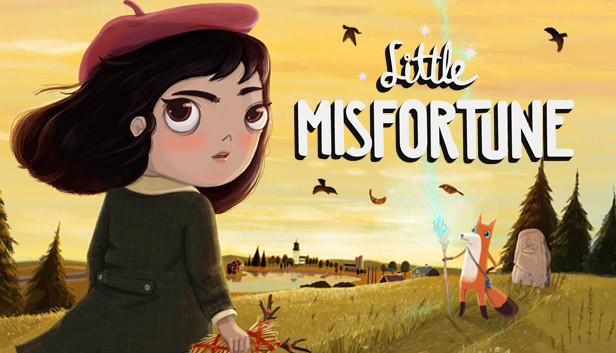
\includegraphics[width=0.6\textwidth, height=0.2\textheight]{Images/little_misfortune.jpg}
  \caption{Little Misfortune จากเว็บไซต์}\label{little_misfurtune}
\end{figure}

\subsection{Martha is dead}
\subsubitem \textbf{Martha is dead} \cite{home-sweet-home:theory} เป็นเกมแนว First Person, Psychological Horror เกมนี้จะอยู่ในช่วงเวลาหลังสงครามโลกครั้งที่ 2 โดยผู้เล่นจะได้รับบทเป็น Giulia เนื้อเรื่องจะปูมาว่า Giulia มีฝาแฝดที่ชื่อว่า Martha ซึ่ง Martha เป็นลูกที่พ่อแม่รักมาก ๆ ต่างกับ Giulia ที่มีแต่ความเกลียดชัง อยู่มาวันหนึ่ง Martha ได้เสียชีวิตลงที่กลางทะเลสาย หลังจากนั้น Giulia ก็ต้องสืบหาความจริงว่าเกิดอะไรขึ้นกับ Martha โดยการปลอมตัวเป็น Martha และเธอก็ได้พบกับเรื่องราวต่าง ๆ มากมาย และภายหลังเกมก็จะค่อย ๆ เฉลยว่า จริงๆแล้ว Giulia ไม่ใช่ฝาแฝด แต่เป็นอีกบุคลิกที่ Martha สร้างขึ้นมาเพื่อหลบหนีจากความรุนแรงที่แม่ของเธอเคยทำร้ายเธอตอนเด็ก ๆ ซึ่งส่งผลให้ Martha นั้นมีบุคลิกที่คล้ายกับคนเป็นใบ้ หูหนวก ซึ่งต่างจาก Giulia ที่เป็นคนปกติ
\begin{figure}[h]
  \centering
  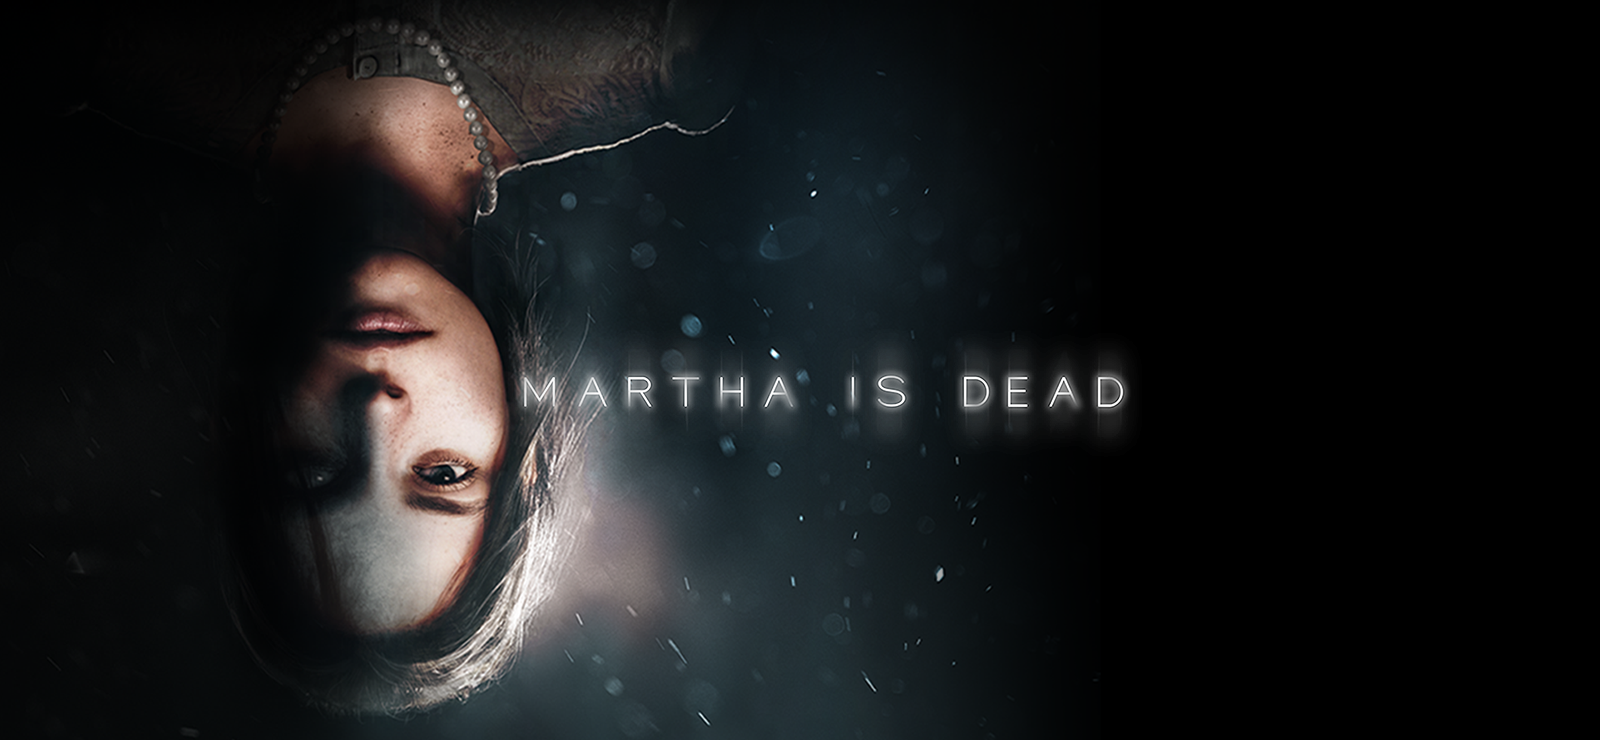
\includegraphics[width=0.6\textwidth, height=0.2\textheight]{Images/martha_is_dead.png}
  \caption{Martha is dead จากเว็บไซต์}\label{martha_is_dead}
\end{figure}
% \subsubsection{Subsubsection 2 heading goes here}
% Subsubsection 2 text

% \subsubsection{Subsubsection 2 heading goes here}
% Subsubsection 2 text

\section{โปรแกรมที่เกี่ยวข้อง}
\subsection{Unity Editor}
\subsubitem \textbf{Unity Editor} \cite{unity:program} เป็นโปรแกรมที่ใช้ในการพัฒนาวอฟต์แวร์และการจำลองต่างๆ เช่น เกม ภาพยนต์ แอนิเมชั่น เป็นต้น ซึ่งใช้ภาษา C$\#$ เป็นหลัก ทั้งนี้ Unity ยังมี Unity asset store พื้นที่ที่ใช้ในการ ซื้อ-ขายชิ้นงาน
\begin{figure}[h]
  \centering
  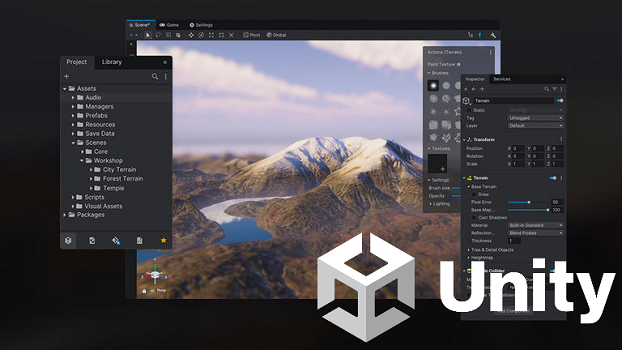
\includegraphics[width=0.6\textwidth, height=0.2\textheight]{Images/unity-engine-landscape-swimlane.png}
  \caption{Unity Editor จากเว็บไซต์}\label{Unity}
\end{figure}

\subsection{Microsoft Visual Studio}
\subsubitem \textbf{Microsoft Visual Studio} \cite{microsoft-visual-studios:program} เป็น IDE ที่ถูกพัฒนาขึ้นโดย Microsoft เป็นเครื่องมือที่ช่วยนักพัฒนาซอฟต์แวร์พัฒนาโปรแกรมคอมพิวเตอร์ เว็บไซต์ เว็บแอปพลิเคชั่น และเว็บเซอร์วิซ
\begin{figure}[h]
  \centering
  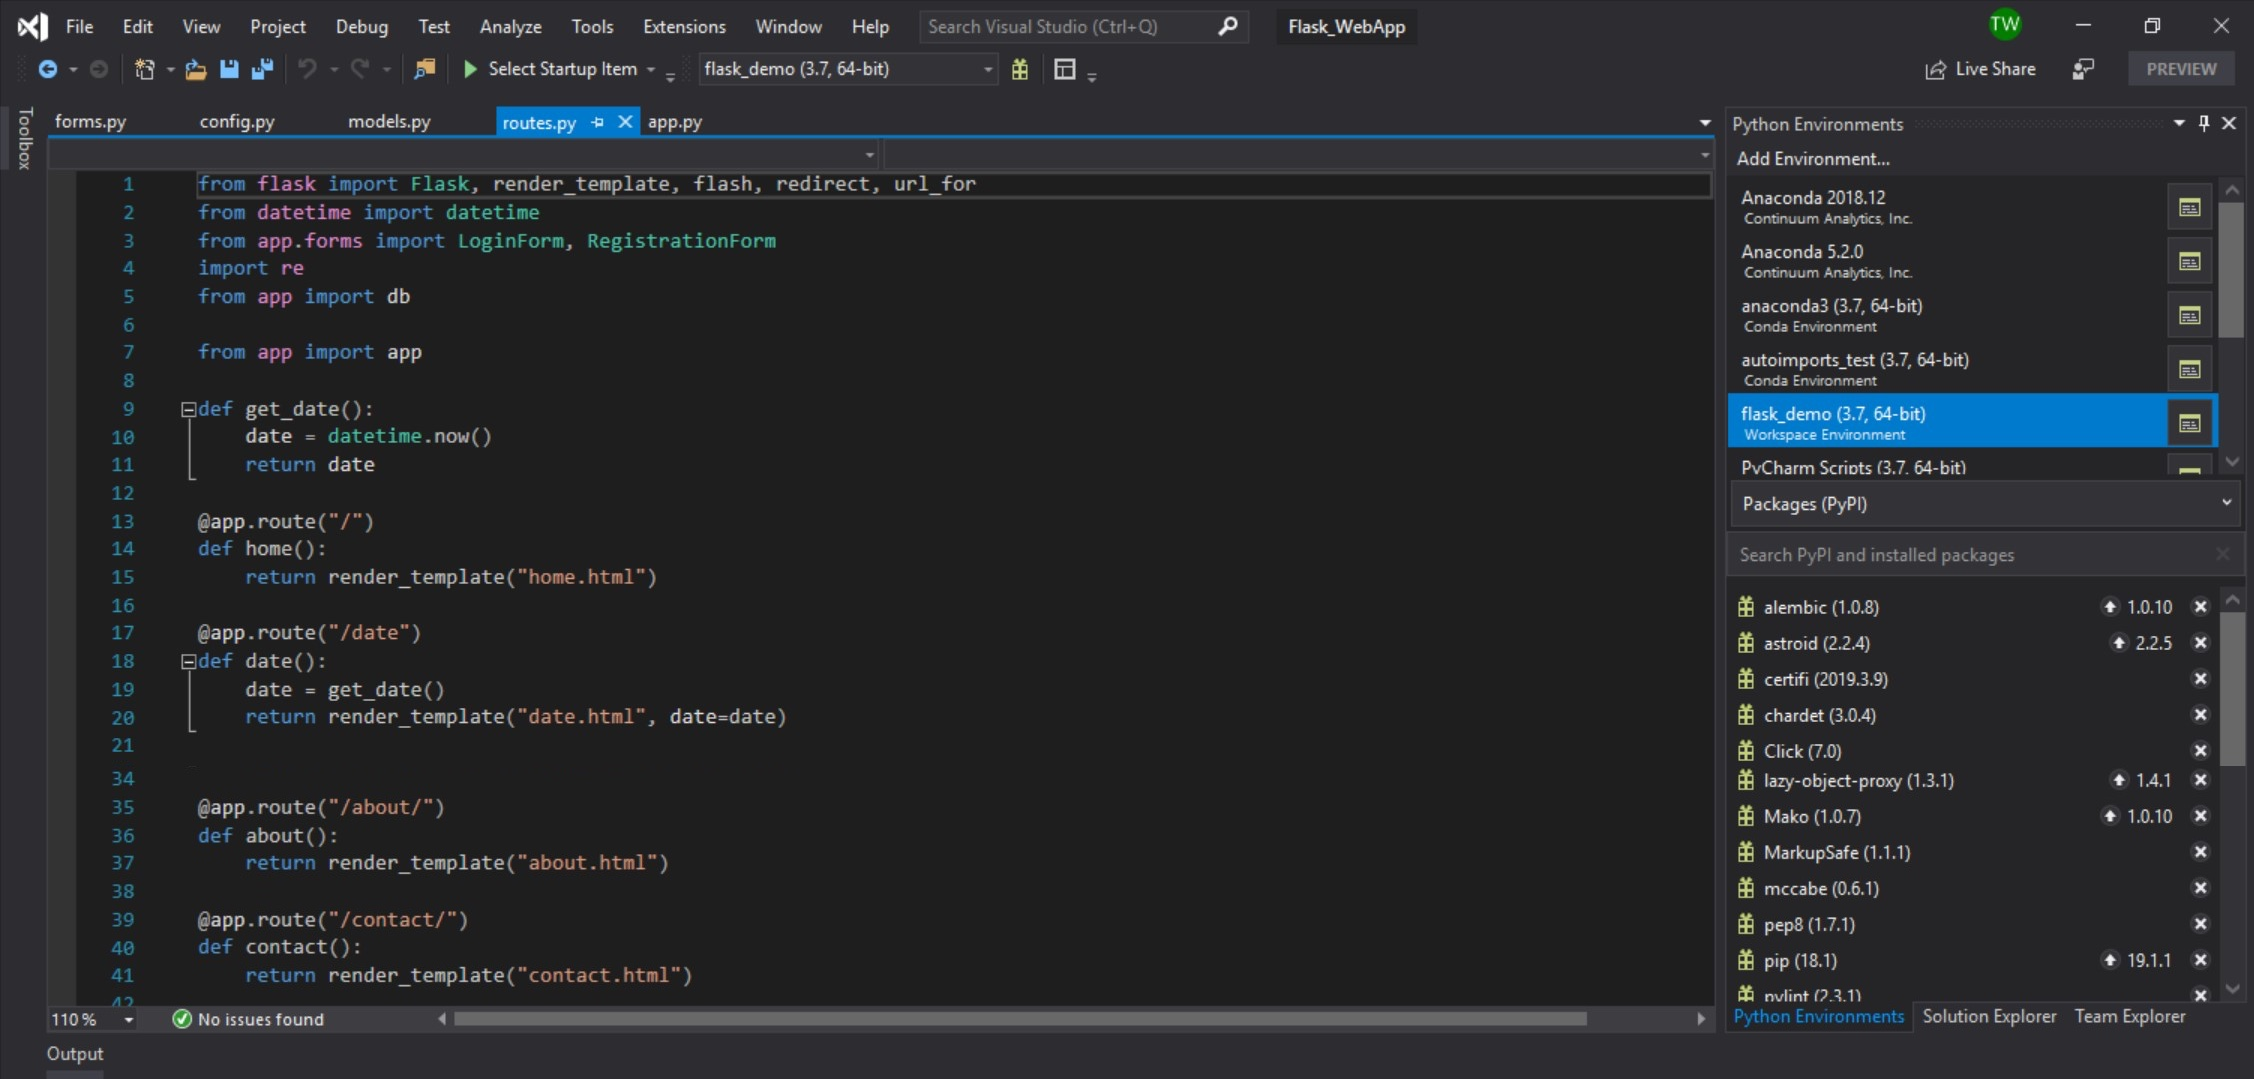
\includegraphics[width=0.6\textwidth, height=0.2\textheight]{Images/python-development-cropped.jpg}
  \caption{Microsoft Visual Studio จากเว็บไซต์}\label{Microsoft}
\end{figure}

\subsection{Jira}
\subsubitem \textbf{Jira} \cite{jira:program} เป็นแอปพลิเคชั่นที่พัฒนาโดย Atlassian ช่วยให้ติดตามความคืบหน้าของงานและจุดบกพร่อง และยังช่วยให้โครงการมีความคล่องตัวมากขึ้น
\begin{figure}[h]
  \centering
  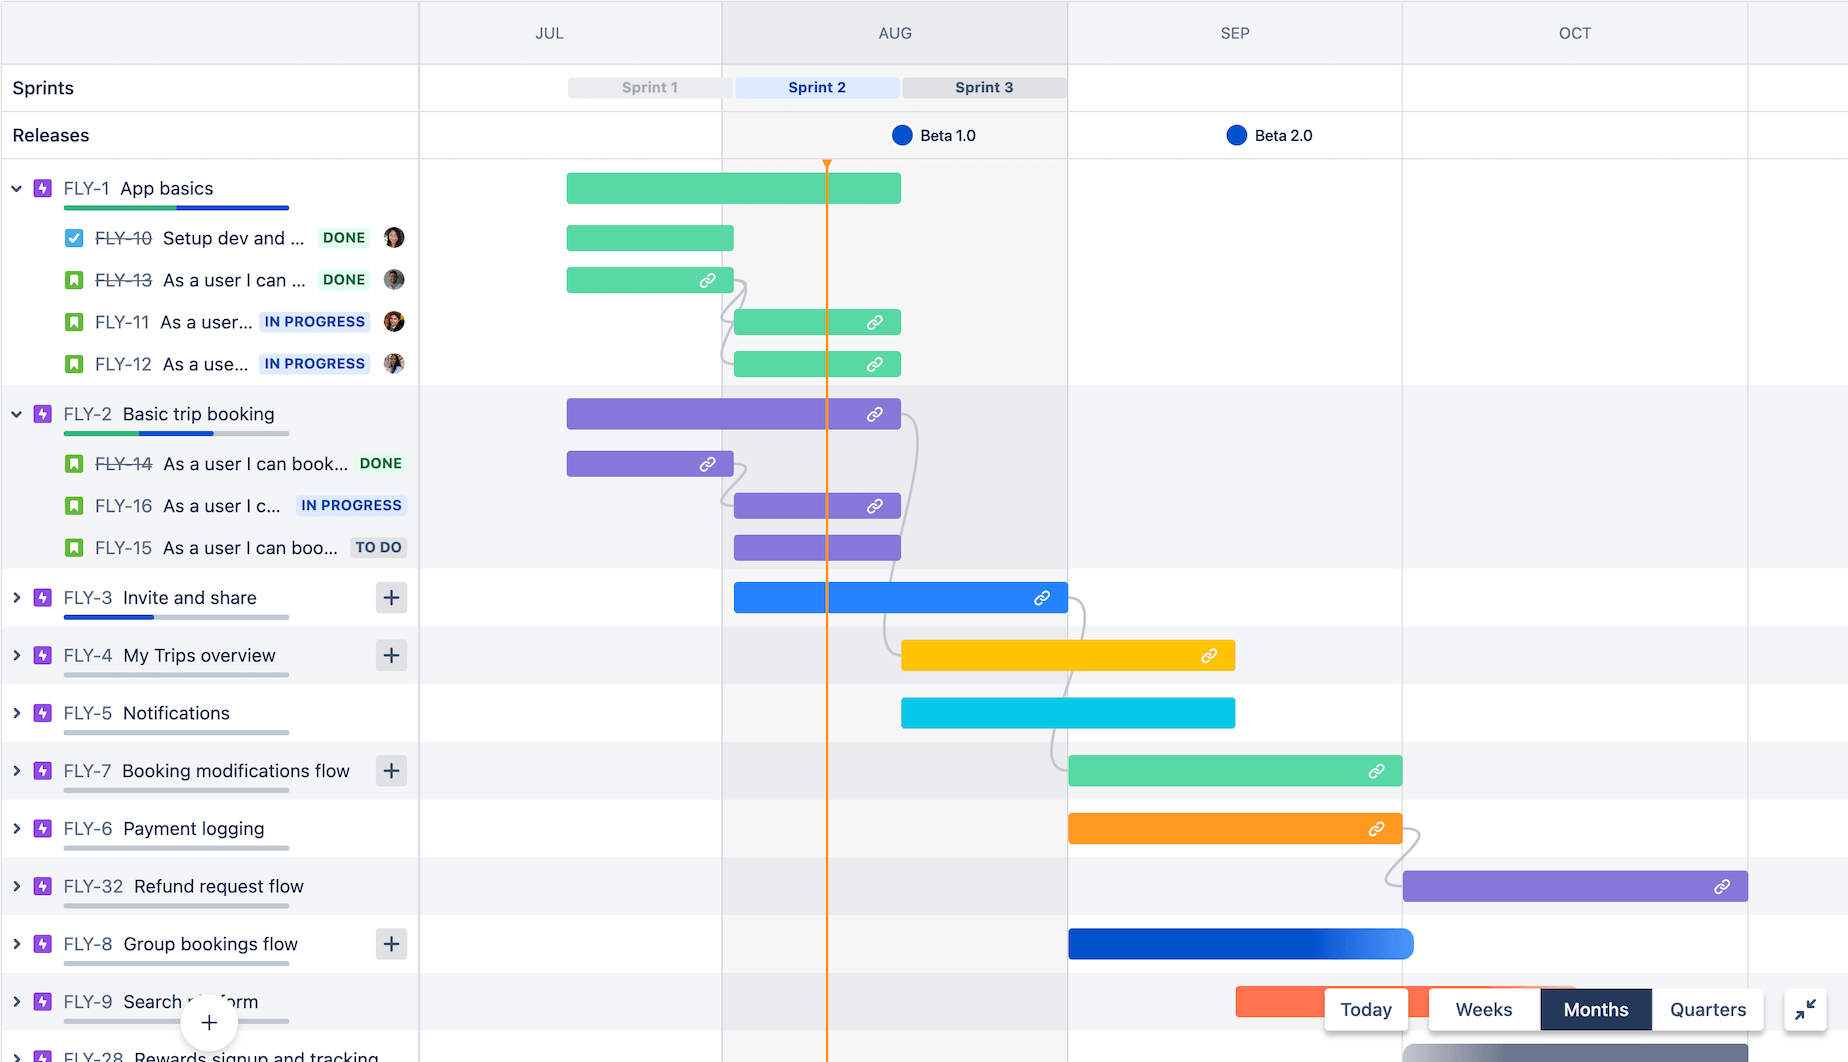
\includegraphics[width=0.6\textwidth, height=0.2\textheight]{Images/screen-roadmaps.png}
  \caption{Jira Platform จากเว็บไซต์}
\end{figure}

\subsection{Unity Asset Store}
\subsubitem \textbf{Japanese School - Stylized} \cite{japanese-school:asset} ใช้ในการสร้างฉากโรงเรียน โดยนำส่วนประกอบต่างๆ มาประกอบร่างกัน
\begin{figure}[h]
  \centering
  \includegraphics[width=0.6\textwidth, height=0.2\textheight]{Images/c7836435-cb4d-4b89-9620-466dbdd5a403_orig.png}
  \caption{Japanese School - Stylized จากเว็บไซต์}\label{JapaneseSchool}
\end{figure}
\newline
\subsubitem \textbf{Casual 1 - Anime Girl Characters} \cite{anime-girl:asset} ใช้เป็น Main Character ในรุ่นทดลอง
\begin{figure}[h]
  \centering
  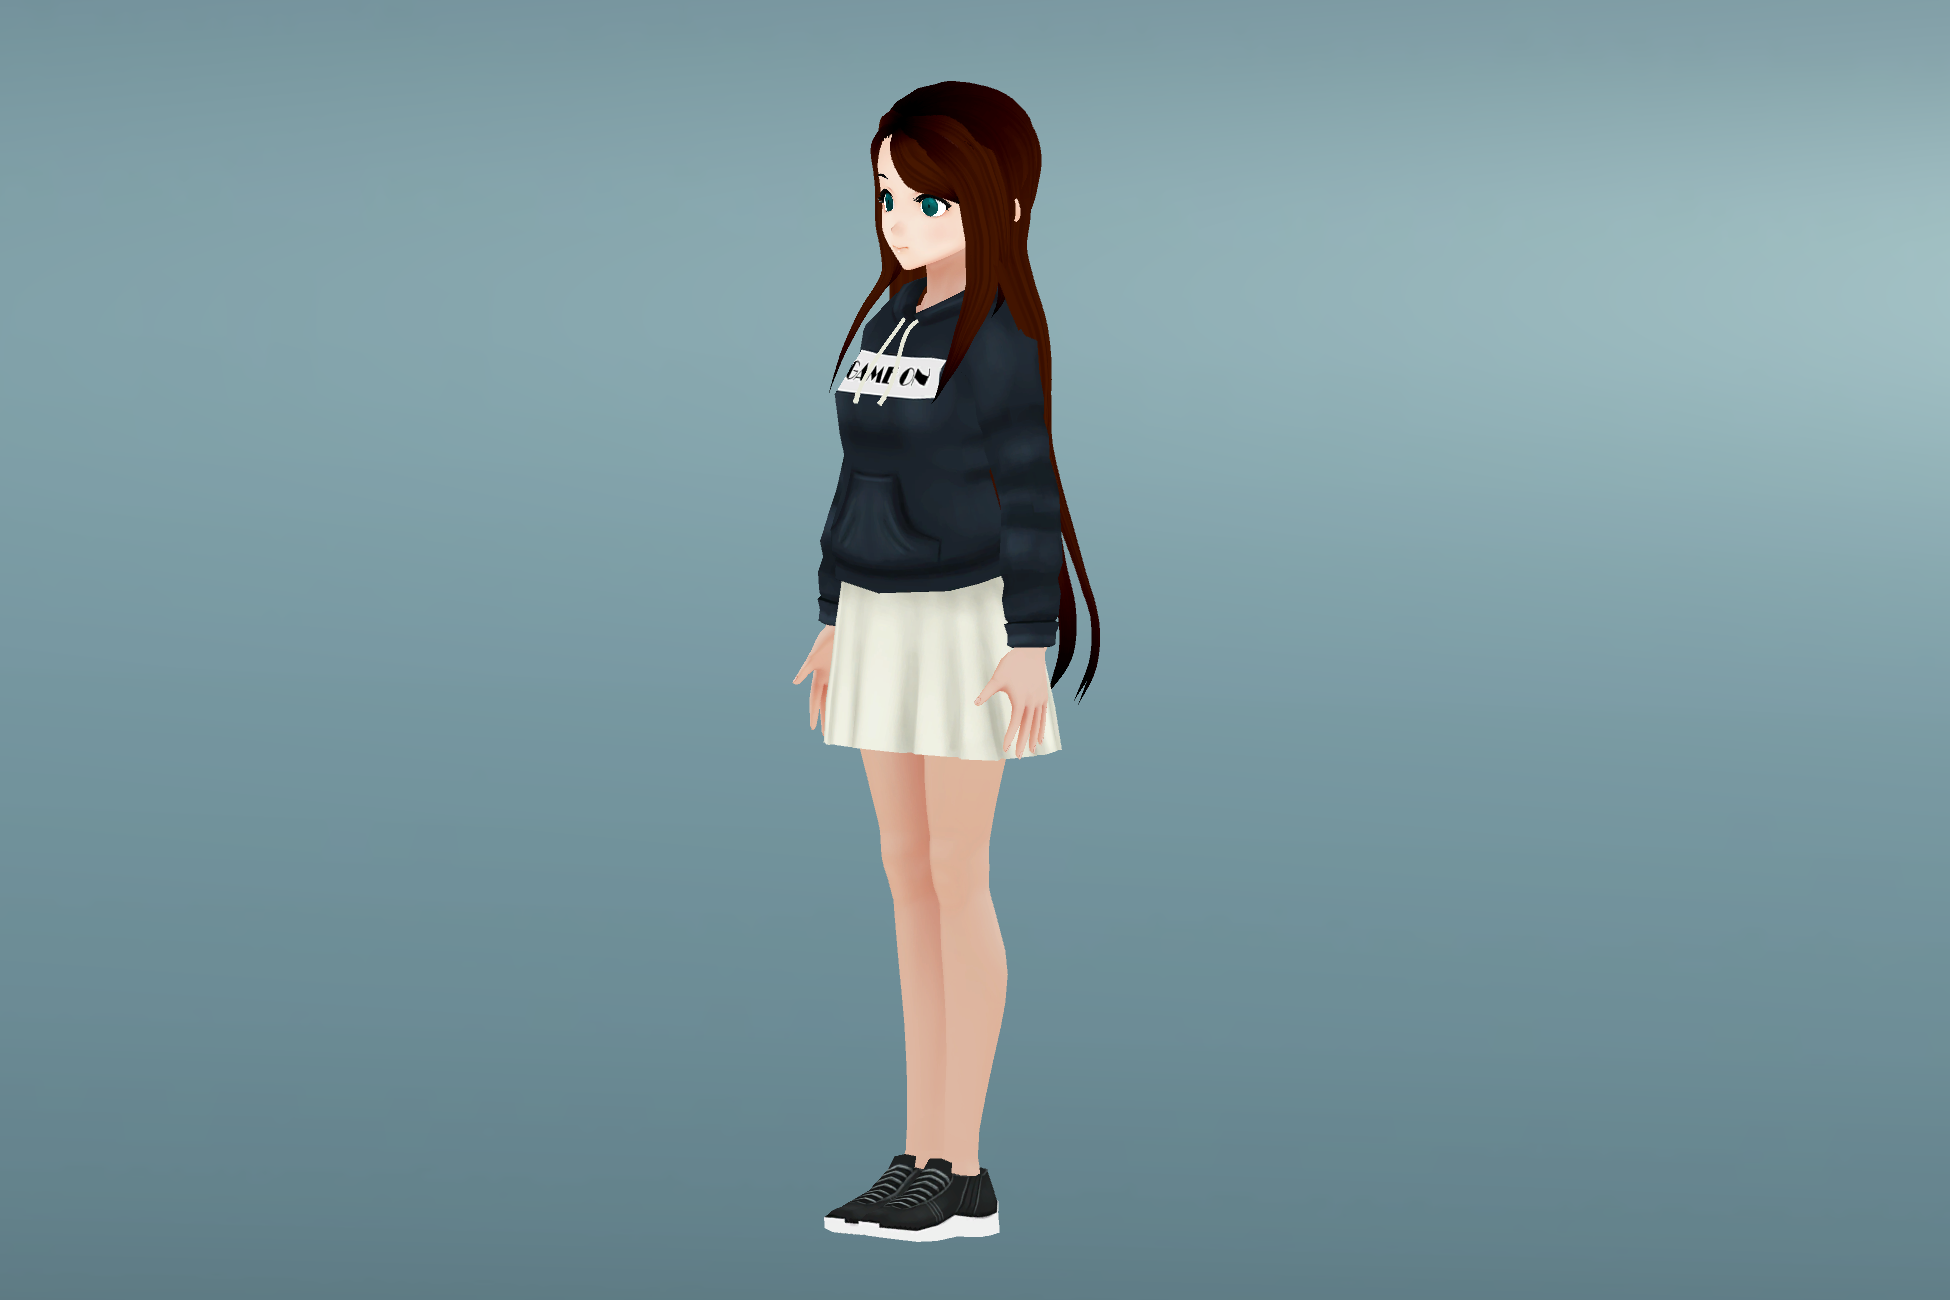
\includegraphics[width=0.6\textwidth, height=0.2\textheight]{Images/7c8d1857-1f28-440d-a966-2c09fe1db214_orig.png}
  \caption{Casual 1 - Anime Girl Characters จากเว็บไซต์}\label{AnimeGirl}
\end{figure}
\newline

% Section 3 text. The dielectric constant\index{dielectric constant}
% at the air-metal interface determines
% the resonance shift\index{resonance shift} as absorption or capture occurs
% is shown in Equation~\eqref{eq:dielectric}:

% \begin{equation}\label{eq:dielectric}
% k_1=\frac{\omega}{c({1/\varepsilon_m + 1/\varepsilon_i})^{1/2}}=k_2=\frac{\omega
% \sin(\theta)\varepsilon_\mathit{air}^{1/2}}{c}
% \end{equation}

% \noindent
% where $\omega$ is the frequency of the plasmon, $c$ is the speed of
% light, $\varepsilon_m$ is the dielectric constant of the metal,
% $\varepsilon_i$ is the dielectric constant of neighboring insulator,
% and $\varepsilon_\mathit{air}$ is the dielectric constant of air.

% \section{About using figures in your report}

% define a command that produces some filler text, the lorem ipsum.
\newcommand{\loremipsum}{
  \textit{Lorem ipsum dolor sit amet, consectetur adipisicing elit, sed do
    eiusmod tempor incididunt ut labore et dolore magna aliqua. Ut enim ad
    minim veniam, quis nostrud exercitation ullamco laboris nisi ut
    aliquip ex ea commodo consequat. Duis aute irure dolor in
    reprehenderit in voluptate velit esse cillum dolore eu fugiat nulla
    pariatur. Excepteur sint occaecat cupidatat non proident, sunt in
    culpa qui officia deserunt mollit anim id est laborum.}\par}

% \begin{figure}
%   \centering

%   \fbox{
%      \parbox{.6\textwidth}{\loremipsum}
%   }

%   % To include an image in the figure, say myimage.pdf, you could use
%   % the following code. Look up the documentation for the package
%   % graphicx for more information.
%   % \includegraphics[width=\textwidth]{myimage}

%   \caption[Sample figure]{This figure is a sample containing \gls{lorem ipsum},
%   showing you how you can include figures and glossary in your report.
%   You can specify a shorter caption that will appear in the List of Figures.}
%   \label{fig:sample-figure}
% \end{figure}

% Using \verb.\label. and \verb.\ref. commands allows us to refer to
% figures easily. If we can refer to Figures
% \ref{fig:walrus} and \ref{fig:sample-figure} by name in the {\LaTeX}
% source code, then we will not need to update the code that refers to it
% even if the placement or ordering of the figures changes.

% \loremipsum\loremipsum

% This code demonstrates how to get a landscape table or figure. It
% uses the package lscape to turn everything but the page number into
% landscape orientation. Everything should be included within an
% \afterpage{ .... } to avoid causing a page break too early.
% \afterpage{
%   \begin{landscape}
%   \begin{table}
%     \caption{Sample landscape table}
%     \label{tab:sample-table}

%     \centering

%     \begin{tabular}{c||c|c}
%         Year & A & B \\
%         \hline\hline
%         1989 & 12 & 23 \\
%         1990 & 4 & 9 \\
%         1991 & 3 & 6 \\
%     \end{tabular}
%   \end{table}
%   \end{landscape}
% }

% \loremipsum\loremipsum\loremipsum

% \section{Overfull hbox}

% When the \verb.semifinal. option is passed to the \verb.cpecmu. document class,
% any line that is longer than the line width, i.e., an overfull hbox, will be
% highlighted with a black solid rule:
% \begin{center}
% \begin{minipage}{2em}
% juxtaposition
% \end{minipage}
% \end{center}
\section{\ifenglish%
    \ifcpe CPE \else ISNE \fi knowledge used, applied, or integrated in this project
  \else%
    ความรู้ตามหลักสูตรซึ่งถูกนำมาใช้หรือบูรณาการในโครงงาน
  \fi
 }

% อธิบายถึงความรู้ และแนวทางการนำความรู้ต่างๆ ที่ได้เรียนตามหลักสูตร ซึ่งถูกนำมาใช้ในโครงงาน
\begin{itemize}
  \item \textbf{Object-Oriented programming} ออกแบบโครงสร้างหลักของการเขียนโปรแกรม การตั้งค่าองค์ประกอบต่างๆ และการเขียนโปรแกรมเชิงวัตถุ
  \item \textbf{Algorithms} ใช้ในการออกแบบ logic เพื่อเพิ่มประสิทธิภาพในการทำงานหรือการคำนวนของ function
  \item \textbf{Software Engineering} ใช้หลักการการพัฒนาซอฟต์แวร์อย่างเป็นระบบ ในการพัฒนาเกมขึ้นมา
  \item \textbf{HCI} ใช้ในการปรับปรุงหน้าตาของระบบเพื่อให้ ผู้เล่นเข้าใจได้ง่าย
\end{itemize}

\section{\ifenglish%
    Extracurricular knowledge used, applied, or integrated in this project
  \else%
    ความรู้นอกหลักสูตรซึ่งถูกนำมาใช้หรือบูรณาการในโครงงาน
  \fi
 }

% อธิบายถึงความรู้ต่างๆ ที่เรียนรู้ด้วยตนเอง และแนวทางการนำความรู้เหล่านั้นมาใช้ในโครงงาน
\begin{itemize}
  \item \textbf{Unity Library} เรียนรู้การใช้งาน Unity และการทำงานของตัว library เป็นหัวใจหลักในการใช้องค์ความรู้จากการศึกษามาพัฒนาเกม
  \item \textbf{Game Design} เรียนรู้การออกแบบระบบให้กับการพัฒนาเกมให้มีความสมบูรณ์
  \item \textbf{Graphics Design} เรียนรู้การออกแบบและจัดวางองค์ประกอบ เพื่อที่จะนำไปใช้ในการออกแบบองกค์ประกอบของภาพ และความกลมกลืน
\end{itemize}
